% The below lines indicate the class and packages used in this Document
\documentclass[a4paper,12pt]{article}
\usepackage[utf8]{inputenc}
\usepackage{graphicx}
\usepackage{geometry}
% This is used for hiding the red-color border boxes appearing on the hyperlink in the Table Of Contents in the previous version
\usepackage[hidelinks]{hyperref}
% This is used for drawing FlowChart Representation of Function Calls in script.js 
\usepackage{tikz}
\usetikzlibrary{shapes.geometric, arrows}
% This is used for adding a header and footer to these pages
\usepackage{fancyhdr}
\pagestyle{fancy}

% Styling for the Header and Footer:
\renewcommand{\headrulewidth}{0.4pt}
\renewcommand{\headwidth}{\textwidth}
\fancyhead[L]{CS 104 Project: Howzatt! Cricket Scorekeeper}
\fancyhead[R]{\makebox[\textwidth][r]{Harsha Vardhan}}
\fancyfoot[C]{\thepage}

% This is a command from the geometry package that is used to customize the margin 
\geometry{margin=1in}
% This is for setting up the styles to be used in the flowchart
\tikzstyle{startstop} = [rectangle, rounded corners, minimum width=3cm, minimum height=1cm,text centered, draw=black, fill=red!30]
\tikzstyle{process} = [rectangle, minimum width=3cm, minimum height=1cm, text centered, draw=black, fill=blue!30]
\tikzstyle{decision} = [diamond, aspect=2, minimum width=3cm, minimum height=1cm, text centered, draw=black, fill=green!30]
\tikzstyle{arrow} = [thick,->,>=stealth]

% This block contains the Title, and information regarding the author of this Document
\title{\textbf{Cricket Webpage Project Documentation}}
\author{Harsha Vardhan \\
Roll Number: 24b1069 \\
IIT Bombay}
\date{\today}

% This is the beginning of the Document 
\begin{document}

\maketitle
\tableofcontents
\newpage

% This is the Introduction for this project, this is referred from the project problem statement provided  
\section{Introduction}
This project involves building a simple live cricket-scoring web application using HTML, CSS, and JavaScript. 
The web app will allow a scorer to input match events (runs, extras, wickets, etc.) using buttons,
and the website will automatically update player and match statistics in real time.

\section{Objectives}
\begin{itemize}
\item To create an intuitive and responsive cricket webpage.
\item To implement navigation through various sections like Teams, Scores, and Tables across various pages such as Setup, Live, Scorecard and Summary.
\item To enhance user experience using consistent UI and responsive design elements.
\end{itemize}

\section{Tools Used}
\begin{itemize}
\item \textbf{Frontend:} HTML, CSS, JavaScript
\item \textbf{IDE:} VS Code
\item \textbf{Testing:} Selenium Module in Python
\item \textbf{Version Control:} GitHub \\
 Repository: \url{https://github.com/Y-Harsha-Vardhan/CS104-Project.git}
\end{itemize}

\section{Project Structure}
\vspace{0.3cm}
\begin{description}
\item [\texttt{script.js}] --- Contains all JS Logic for the project
\item [\texttt{setup.html}] --- HTML page for entering the data about the teams
\item [\texttt{setup.css}] --- Styling for the setup.html page
\item [\texttt{live.html}] --- HTML page for controlling and viewing the score of the match
\item [\texttt{live.css}] --- Styling for the live.html page
\item [\texttt{scorecard.html}] --- HTML page for the scorecard of the match upto that point
\item [\texttt{scorecard.css}] --- Styling for the scorecard.html page 
\item [\texttt{summary.html}] --- HTML page for displaying the result at the end of the match 
\item [\texttt{summary.css}] --- Styling for the summary.html page
\item [\texttt{Images/}] --- This folder contains the images used in the webpage
\item [\texttt{autofill.py}] --- This is a python script that helps to automatically fill the data in the \hspace*{2cm} webpage, here I used this for testing the working of the website.
\end{description}
\clearpage

\section{Design and Layout}
The following are the screenshots of various pages of the Website:
\begin{figure}[h!]
\centering
\includegraphics[width=\textwidth]{images/homepage.png}
\caption{Homepage of the Cricket Webpage}
\label{homepage}
\end{figure}

\begin{figure}[h!]
\centering
\includegraphics[width=\textwidth]{images/live-modal.png}
\caption{The initial modal on the Live Page}
\label{live-modal}
\end{figure}
\clearpage

\begin{figure}[h!]
\centering
\includegraphics[width=\textwidth]{images/live.png}
\caption{Live Page of the Cricket Webpage}
\label{live}
\end{figure}

\vspace{1.5cm}

\begin{figure}[h!]
\centering
\includegraphics[width=\textwidth]{images/scorecard.png}
\caption{Scorecard Page of the Cricket Webpage}
\label{scorecard}
\end{figure}

\begin{figure}[h!]
\centering
\includegraphics[width=\textwidth]{images/summary.png}
\caption{Summary Page of the Cricket Webpage}
\label{summary}
\end{figure}  

\section{Basic Features}
\begin{enumerate}
\item Setup page allows user to enter team names, toss winner and toss decision \hyperref[homepage]{[Fig 1]}.
  \begin{itemize}
  \item This is done using the following functions: \textit{startMatch()}
  \item Click on this to see more about the above function in detail: \hyperref[basic1]{Setup Page}
  \end{itemize}
\item Live page allows the user to control the match using buttons ( [Runs-0,1,2,3,4,6] [Wicket] ) and updates the display (that shows the Strike, Non-Strike Batters, Current Bowler Stats; CRR, RRR and Current Over data) dynamically [Fig \ref{live-modal}, \ref{live}].
  \begin{itemize}
  \item This is done using the following functions: \textit{loadMatchData()}, \textit{setUpEventListeners()}, \textit{updateDisplay()} and \textit{promptForPlayerNames()}
  \item There are other sub-functions also that are called from these main functions, click on this to check out the function flow: \hyperref[flowchart]{FlowChart Representation}
  \item Click on this to see more about the above functions and sub-functions in detail: \hyperref[basic2]{Live Page}
  \end{itemize}
\item Scorecard page shows the match data of all the players until that point of the match in a tabular format \hyperref[scorecard]{[Fig 4]}.
  \begin{itemize}
  \item This is done using the following functions: \textit{goBack()}, \textit{formatOvers(balls)}, \textit{loadScoreCard()} and \textit{setupCommentaryHover()}
  \item Click on this to see more about the above functions in detail: \hyperref[basic3]{Scorecard Page}
  \end{itemize}
\item Summary page displays the final match result and allows the user to Reset the match or View Scorecard if required \hyperref[summary]{[Fig 5]}.
  \begin{itemize}
  \item This is done using the following functions: \textit{displayResult()} and \textit{setupSummaryPage()}
  \item Click on this to see more about the above functions in detail: \hyperref[basic4]{Summary Page}
  \end{itemize}
\end{enumerate}

\section{Customizations (Click on the function's names to see more about them:)}
\begin{enumerate}
\item Can Set Custom Number of Overs for a Match (by default if nothing is given, it remains 2 per Innings)
  \begin{itemize}
  \item For this feature, I added an additional label and input field after the ones required for the Basic Part in the Setup Page Container
  \item It only accepts numbers, not strings.
  \item If nothing is entered or an invalid number such as (-1) is entered then it takes 2 as the value.
  \item It stores this value in the \textit{teamData} object along with the other data.
  \end{itemize}
\item Wide, No Ball and Run Out Buttons Functionality 
  \begin{itemize}
  \item The Wide Functionality is implemented by: \hyperref[wide]{\textit{addWide()}} 
  \item The No Ball Functionality is implemented by: \hyperref[noBall1]{\textit{addNoBall()}} and \hyperref[noBall2]{\textit{consumeFreeHitIfNotExtra()}} \\ It shows a Free Hit Indicator after a No Ball and removes it after the next valid delivery
  \item The Run Out Functionality is implemented by: \hyperref[runOut1]{\textit{promptForRunOut()}} and \hyperref[runOut2]{\textit{processRunOut()}}
  \end{itemize}
\item Commentary in Scorecard Page when hovering on a player's stats
  \begin{itemize}
  \item This is done using the function: \hyperref[commentaryHover]{\textit{setupCommentaryHover()}}
  \item It uses (mouseenter) and (mouseleave) EventListeners to show and hide the commentaries
  \item The commentaries are in the ball-by-ball log format: (Eg: 2.3 Bumrah to Head, 2 runs) 
  \end{itemize}
\item Error Handling for the Player Names (preventing duplicate names)
  \begin{itemize}
  \item This depends on the functions: \hyperref[error1]{\textit{isDuplicatePlayer()}}, \hyperref[error2]{\textit{showModalError()}}
  \item The usage of this Customization is to show an Error Message in the Modal, when an Invalid Player's Name is entered
  \item This message disappears once the User starts typing again.
  \end{itemize}
\item An automated Python Script that runs the match
  \begin{itemize}
  \item This is written in the file: \texttt{autofill.py} and is based on the Selenium Module in Python
  \item To Run this file in your device, you need to: SetUp a Driver for your preferred Browser, and Specify the path of the file in your PC.
  \item This file simulates a match between RCB and CSK (as given as an example in the Problem Statement), it also uses random module to select an action to perform or select a new player's name.
  \item It stores the names of the players in respective lists of teams and maintains a set which contains the names of the players who have already played and hence prevents the repetition of player names while using random.
  \item It consists of the following helper functions:
    \begin{description}
      \item [\texttt{fill\_starting\_players(batters, bowlers)}]: \\ --- Enters the names of the players in the beginning of an innings
      \item [\texttt{fill\_new\_batter()}]: \\ --- Enters the name of the next batsman after a Wicket
      \item [\texttt{fill\_new\_bowler()}]: \\ --- Enters the name of the next bowler after an Over
      \item [\texttt{click\_action(action)}]: \\ --- Simulates the clicking of the Control Buttons randomly. \\ --- It uses weights to adjust the randomness of a particular clickAction \\ --- It also has a checking mechanism to prevent unnatural scenarios like \hspace*{0.45cm} all Wides or all Wickets in an over \\ --- Currently it ensures that the maximum numbers in an over are: \\ \hspace*{0.45cm} 1 Wide, 1 No Ball, 2 Wickets
    \end{description}
  \item This file also prints the output of each ball into the terminal, and requires the User to click the Continue Buttons in the Innings Break and at the End of The Match.
  \item In the End the Page redirects to the Summary Page, from which you can View the Scorecard or Reset Match before the window closes (Currently it closes 100 seconds after the match has ended)
  \item The following is a clickable template that will redirect to a video showing this:
  \end{itemize}
\end{enumerate}
\begin{figure}[h]
  \centering
  \href{https://drive.google.com/file/d/1Z6U6ZtFrIRRqnZfjVCqRuwvF0Dh_1dh4/view?usp=sharing}{
    
\includegraphics[width=0.6\textwidth]{images/autofillDemo.png}
  }
  \caption{Click to watch the AutoFill Demo}
\end{figure}


\section{Functions Used in JS: \textit{score.js}}

\subsection{Setup Page:}
\label{basic1}
\subsubsection{\textit{startMatch()}}
\begin{itemize}
\item Gets the names of the 2 teams, that are entered by the user and stores them in respective variables.
\item Similarly, stores the name of the team that has won the toss (decided by user) and what that team's decision is (either to \textbf{bat} or to \textbf{bowl}).
\item Allows the user to enter custom input for number of overs, if not entered or invalid input then defaults to 2 overs.
\item Shows error messages if the user tries to submit without filling all the fields or if the two team's names are the same.
\item Stores all these variables in an object: \textit{teamData}
\item Next it stores this object in the browser's \textit{localStorage} by converting it into a \textit{JSON String}.
\item It clears any potentially leftover data: \textit{cricketMatchData} from the \textit{localStorage} of the browser.
\item Finally it redirects to the Live Page.
\end{itemize}

\subsection{Live Page:}
\label{basic2}
When this page is initialized, an \textit{EventListener} calls: \textit{loadMatchData()} and \textit{setupEventListeners()}, 
if the match isn't over and players are not yet set up, it calls \textit{promptForPlayerNames()} else it calls \textit{updateDisplay()}.
\subsubsection{\textit{loadMatchData()}}
\begin{itemize}
\item It gets the match data that is stored as \textit{cricketMatchData} in the \textit{localStorage}.
\item It stores it in a \textit{matchData} object. 
\end{itemize}

\subsubsection{\textit{setupEventListeners()}}
\begin{itemize}
\item It calls the function \textit{addRuns()} when a Run Button is clicked.
\item It calls \textit{takeWicket()} when the Wicket Button is clicked.
\item It calls \textit{addWide()} when the Wide Button is clicked.
\item It calls \textit{promptForRunOut()} when the Run Out Button is clicked.
\item It calls \textit{addNoBall()} when the No Ball Button is clicked.
\item It redirects to Scorecard Page when the View Scorecard Button is clicked. 
\item It calls \textit{submitPlayerNames()} when the Submit Names Button is clicked in the \textit{Modal}.
\end{itemize}

\subsubsection{\textit{promptForPlayerNames()}}
\begin{itemize}
\item It calls \textit{showNamePrompt()} with a list as an argument according to the current match status. 
\item In the beginning of the First Innings, these are passed: Strike Batter, Non-Strike Batter, Bowler.
\item In the beginning of the Second Innings, these are passed: Strike Batter, Non-Strike Batter, Opening Bowler.   
\end{itemize}

\subsubsection{\textit{showNamePrompt()}}
\begin{itemize}
\item It sets the \textit{modal} style to flex from none (to make it visible), and makes the \textit{nameInputs} innerHTML attribute to an empty string.
\item It uses the argument it got from \textit{showNamePrompt()} function and adjusts the text for the fields
\item Creates a label for the input fields by adding a ':' to each element of the argument list, and appends it to \textit{nameInputs}
\item It then creates the corresponding input fields with respective ids, and adds a placeholder text.
\item It updates \textit{modalTitle} based on whether it is the First or Second Innings to the appropriate title.
\end{itemize}

\subsubsection{\textit{showModal(title,message,callback)}}
\begin{itemize}
\item This function is used to populate the content of a custom modal.
\item This custom modal present in the Live Page is used to let the user know if the First Innings or the Match has ended.
\item The arguments \textit{title} and \textit{message} are used to populate the \textit{custom\_modal-title} and \textit{custom\_modal-message} respectively.
\item The modal has a Continue Button with id \textit{continue} to Resume the Match, the \textit{callback} argument is used to call a particular function when the Continue Button is clicked.  
\end{itemize}

\subsubsection{\textit{showModalError(message)}}
\label{error2}
\begin{itemize}
\item This function takes the argument \textit{message} and displays it on a modal.
\item It creates an \textit{errorElement} with an id and \textit{textContent} as \textit{message} argument, and it is also styled to make it look like an error.
\item It then appends it to the Modal on the page
\item If any input is being typed after the display of the message, then the message is automatically made empty using an \textit{EventListener}.
\end{itemize}

\subsubsection{\textit{submitPlayerNames()}}
It checks for the correctness of the player names entered, and then stores them
\subsubsection*{This is for the First Innings:}
\begin{itemize}
\item It stores the corresponding data in: \textit{strikeBatter}, \textit{nonStrikeBatter} and \textit{bowler}.
\item If either of the names are missing, it shows an error message in the modal using \textit{showModalError()}.
\item If the entered names of strikeBatter and nonStrikeBatter are same, it shows an error message. 
\item If the entered names are matching the teamNames or if the names are already used in another team, it shows an error.
\item It decides the currentBatting and currentBowling teams based on \textit{matchData} which was initialized in \textit{loadMatchData()} function.
\item It initializes the remaing data such as runs, balls, maidens, overs, etc. of the batsmen and bowlers.
\item It closes the \textit{modal} by setting its display back to none.
\item It calls \textit{saveMatchData()} and \textit{updateDisplay()}.
\end{itemize} 

\subsubsection*{This is for the Second Innings:}
\begin{itemize}
\item It is same as the First Innings for the following: storing data, error handling, and initialising players.
\item It closes the \textit{modal} by setting its display back to none.
\item It calls \textit{saveMatchData()} and \textit{updateDisplay()}.
\end{itemize}

\subsubsection{\textit{isDuplicatePlayer(name,team)}}
\label{error1}
\begin{itemize}
\item This function returns a boolean value.
\item It takes \textit{name} and \textit{team} as arguments and checks if the given name is already used or not.
\item If the function returns true, then that \textit{name} is not valid for that \textit{team} (Eg: batting)
\item And it is valid if it returns false.
\end{itemize}

\subsubsection{\textit{showNewBatterPrompt()}}
\begin{itemize}
\item This function is used to show a prompt when a batsman gets out, and handle the data insertion.
\item It checks if the entered name is valid or not using \textit{isDuplicatePlayer()} and shows error if not.
\item If the name is valid then it adds the name along with the initialized data of the \textit{new-batter} to the \textit{matchData}.
\item Finally, it resets the modal to hidden and calls \textit{saveMatchData()} and \textit{updateDisplay()}.  
\end{itemize}

\subsubsection{\textit{showNewBowlerPrompt()}}
\begin{itemize}
\item This function is used to show a prompt when an over gets completed, to add a new bowler and handles the data insertion.
\item It performs all the functions of \textit{showNewBatterPrompt()} function for bowlers.
\item Additionally, if it is not the End of the Match, then it re-enables the buttons (because they might have been disabled by other functions at this stage)
\end{itemize}

\subsubsection{\textit{checkForEndOfMatchOrInnings()}}
\begin{itemize}
\item It stores the truth values of either the overs completing and all out in: \textit{oversCompleted} and \textit{allOut} respectively.
\item In the first innings, if either \textit{oversCompleted} or \textit{allOut} is true, then it sets \textit{matchData.allOut} to true (The way the functions work, just a convenience), calls \textit{startSecondInnings()} and returns \textit{true} for the function.
\item In the second innings, if target is reached then, it calls \textit{endMatch()} with Result Statement as argument
\item If either the overs are completed or all out, it checks for the possibility of Draw and calls the \textit{endMatch()} with appropriate argument and finally returns true for the function.
\item In any other case, it returns false.
\end{itemize}

\subsubsection{\textit{startSecondInnings()}}
\begin{itemize}
\item This function handles the transition from the first innings to the second.
\item It stores the necessary data like \textit{firstInningsTotal}, \textit{firstInningsWickets}, \textit{firstInningsBatters} in new attributes in the \textit{matchData} object, as the attributes in which the old data is present will be overwritten.
\item It then re-initializes all the attributes of \textit{matchData} for the second innings.
\item It swaps the \textit{currentBowlingTeam} and \textit{currentBattingTeam} and sets the names of the opening batsmen and bowler to \textit{null}.
\item It notifies the user that the first innings has ended with a message that also shows the target for the second innings.
\item It calls \textit{showModal()} with the \textit{message} as innings break and \textit{callback} as \textit{promptForPlayerNames} 
\end{itemize}

\subsubsection{\textit{endMatch(message)}}
\begin{itemize}
\item This function handles the end of match, it sets \textit{matchData.matchOver} to true
\item It populates the \textit{matchData.statusMessage} with the \textit{message} argument it is called with.
\item It calls \textit{saveMatchData()} and \textit{updateDisplay()}.
\item It calls \textit{showModal} with the \textit{message} as Match Over and \textit{callback} as Time-Delay for 2s before redirecting to Summary Page.
\item It disables all the control buttons to prevent any further change.
\end{itemize}

\subsubsection{\textit{addRuns(runs)}}
\begin{itemize}
\item This function updates the scores of batsmen and bowler based on value of the run button clicked, it takes the value of this button as its \textit{runs} argument.
\item It returns (no change) if either: the match is over, all out, or if the \textit{currentStriker} is not properly set (null).
\item It also calls the \textit{consumeFreeHitIfNotExtra(false)} which will remove any Free Hit Indicator message in the Live Match Display.
\item It updates the batter's runs and balls and updates 4s and 6s if required
\item It updates the bowler's stats as well.
\item It updates the \textit{totalRuns} and \textit{balls} of \textit{matchData}.
\item It calls \textit{addCommentary(runs)} with \textit{runs} as argument.
\item It checks for end of match or innings and if true, then calls \textit{saveMatchData()}, \textit{updateDisplay()} and returns.
\item If odd runs are scored or end of over, then it switches the two batter's positions.
\item It also updates the overs of the bowler, if the bowler is valid and he is the \textit{currentBowler}.
\item At the end of an over, if it is not an end of the match or innings, it prompts for the new bowler's name.
\item It calls \textit{saveMatchData()} and \textit{updateDisplay()} outside of all the conditional if-else statements in this function. 
\end{itemize}

\subsubsection{\textit{takeWicket()}}
\begin{itemize}
\item This function updates the data of the bowler and sets the \textit{currentStriker} batsman as out
\item It returns (no change) if either: the match is over, all out, \textit{matchData.wickets} >= 10 or if \textit{currentStriker} is not properly set (null).
\item It calls \textit{consumeFreeHitExtra(false)} which will remove any Free Hit Indicator message in the Live Match Display.
\item It sets the \textit{currentStriker} to out and calls \textit{addCommentary('W')} function
\item It then checks for end of match or innings and if true, then calls \textit{saveMatchData(), updateDisplay()}.
\item If \textit{matchData.wickets < 10} then calls \textit{showNewBatterPrompt()} else it sets \textit{matchData.allOut} to true.
\item It checks for End of Over, and swaps the \textit{currentStriker} and \textit{nonStriker}, updates the bowler stats and calls \textit{showNewBowlerPrompt()}
\item It then adds the new bowler to the list of bowlers in \textit{matchData.bowlers}
\item It finally calls \textit{saveMatchData()} and \textit{updateDisplay()} to update changes.
\end{itemize}

\subsubsection{\textit{addWide()}}
\label{wide}
\begin{itemize}
\item This function updates the player data according to a Wide 
\item It returns (no change) if either: the match is over, all out or \textit{currentBowler} is not properly set (null).
\item It calls \textit{consumeFreehitExtra(true)} so that the Free Hit will carry forward to the next ball as well.
\item It increments the \textit{matchData.extras}, \textit{matchData.totalRuns} and \textit{matchData.currentBowler.runs} by 1 each.
\item It finally calls: \textit{addCommentary('Wd')}, \textit{saveMatchData()} and \textit{updateDisplay()}.
\end{itemize}

\subsubsection{\textit{addNoBall()}}
\label{noBall1}
\begin{itemize}
\item This function is implemented a bit differently compared to conventional No Ball in Cricket Matches
\item It is considered as an extra, and 1 run is awarded to the Batting Team
\item It sets the next ball after a No Ball as a Free Hit and indicates it with an indicator near the display, but the batsman can get RunOut or his Wicket may be taken in this ball if the user presses those buttons.
\item If the next ball is a Wide or a No ball again, then the Free Hit gets carried forward.
\item It calls \textit{consumeFreeHitIfNotExtra(true)}, \textit{addCommentary('Nb')}
\item It sets the \textit{matchData.isFreeHit} to true, and finally calls \textit{saveMatchData()} and \textit{updateDisplay()}.
\end{itemize}

\subsubsection{\textit{consumeFreeHitIfNotExtra(isDeliveryExtra)}}
\label{noBall2}
\begin{itemize}
\item This is a helper function that is used to reset the Match Status after the Free Hit is consumed.
\item It checks if \textit{matchData.isFreeHit} is true, and if \textit{isDeliveryExtra} is false and then sets \textit{matchData.isFreeHit} to false.
\item This is because the ball was a free hit and this delivery is not a Wide or No Ball, so Free Hit is consumed
\item Else, the delivery was an extra and \textit{isFreeHit} remains true.
\end{itemize}

\subsubsection{\textit{promptForRunOut()}}
\label{runOut1}
\begin{itemize}
\item It dynamically creates an Modal Prompt for the user to enter the number of runs that the batter scored before he got out and the name of the new batsman
\item It creates 'Runs scored before out:' and 'New Batter:' labels with their respective input fields and appends them to the modal.
\item It checks the name of the entered new batsman for validity (using \textit{isDuplicatePlayer()}), and then show error if not. It also takes the default value of Runs Scored to be zero if nothing is entered.
\item It calls \textit{processRunOut(runs, newBatter)} and then hides the modal when the Submit Button is clicked.
\item It checks if either the match is not over, not all out, and balls are still left and if all are true then
\item It checks if it is the end of an over and disables all buttons, calls \textit{showNewBowlerPrompt()} to start the next over incase the Run Out is clicked at the end of one over. 
\end{itemize}

\subsubsection{\textit{processRunOut(runs,newBatterName)}}
\label{runOut2}
\begin{itemize}
\item It takes the \textit{runs} and \textit{newBatterName} as arguments, and makes the necessary changes to update the new batsman into the data.
\item It returns (no change) if either: the match is over, all out or if \textit{matchData.wickets} >= 10.
\item It calls the \textit{consumeFreeHitIfNotExtra(false)} and assigns a variable to store the batter object that just got out.
\item It then adds the runs scored before the Run Out, if any to the batter's scores and updates the bowler's and the total match's stats as well.
\item It then sets the \textit{matchData.batters[matchData.currentStriker].out} to true and then pushes the new batter object to \textit{matchData.batters} array and sets his index.
\item It then analyzes the number of runs scored during the run out, to decide which batsman will be the next Strike and Non-Strike batters.
\item It calls \textit{addCommentary(eventCode,details)}, the details has \textit{runs} and \textit{outBatterName} stored in it.
\item It then handles over completion if this was the 6th ball and then calls \textit{saveMatchData()} and \textit{updateDisplay()} to update the data in the Live Page. 
\end{itemize}

\subsubsection{\textit{addCommentary(eventCode,details\{\})}}
\begin{itemize}
\item This function handles the creation of the \textit{matchData.commentary} that contains all the commentaries in a ball to ball format.
\item It ensures that the players are set before before adding commentary and returns (no change) if there is any error in that.
\item It creates objects to store the current batsman at strike and the bowler and checks if they are set correctly.
\item It then depending on the \textit{eventCode} it recieved as an argument, handles it
\item For a Wide or a No Ball, it doesn't count it as a legal delivery and uses the current count for them, for the others it uses the previous count as the ball was just added.
\item It then creates the \textit{description} based on the \textit{eventCode} using a switch-case function and then makes the \textit{commentaryText}
\item It is of the format: OverIndex BowlerName to BatterName, description and then pushes the commenatry to the \textit{matchData.commentary}.
\end{itemize}

\subsubsection{\textit{updateDisplay()}}
It is just a parent function that calls the following functions:
\begin{itemize}
\item \textit{updateScoreDisplay()} : Updates the Score Display in the top of the Live Page \hspace*{4.3cm} Container according to the Innings
\item \textit{updateBattersTable()} : Adds new batsmen, and updates the scores of the batters \hspace*{4.2cm} in the Batter Table
\item \textit{updateBowlerTable()} : Similar as the above function for Bowlers 
\item \textit{updateCrrRrr()} : Calculates and then updates the CRR and RRR depending on \hspace*{3.3cm} the Innings
\item \textit{updateCurrentOver()} : Updates the Current Over section in the Live Page \\ \hspace*{4.1cm} Container using the \textit{matchData.commentary}
\item \textit{updateStatusDisplay()} : A previous iteration of the Webpage, had this function to \hspace*{4.5cm} show the \textit{statusMessage} 
\end{itemize}

\hspace{0.5cm}

The \textit {saveMatchData ()} function stores the \textit {matchData} object as \textit {cricketMatchData} in the \textit {localStorage} of the Web Browser. \\

In the Live Page, there is an \textit{EventListener} that listens to the click of keys and if there are any message-modals in the page, then the user can just press enter instead of manually clicking the button to submit or continue. 

\subsection{Scorecard Page:}
\label{basic3}
For this page there is a small inline script that has an \textit{EventListener}, listening for the \textit{DOMContentLoaded} event.
It calls the \textit{loadScorecard()} function.
\subsubsection{\textit{goBack()}}
This function is called when the Back Button is clicked in the Scorecard Page.
It uses \textit{window.history.back()} to go back to the page before the View Scorecard button was clicked.
If the page is called from the summary, it redirects to the Summary Page and if called from live match, it redirects to Live Page.

\subsubsection{\textit{formatOvers(balls)}}
This function takes \textit{balls} as an argument and returns a corresponding string that represents the number of overs that the bowler has bowled in the match.

\subsubsection{\textit{loadScorecard()}}
\begin{itemize}
\item It first gets the \textit{cricketMatchData} from the \textit{localStorage} of the browser and stores it in \textit{MatchData} object (If it is not there, then the function returns)
\item It then extracts the data of all the batsmen and bowlers who have played until now, and stores them in separate arrays: \textit{firstInningsBatters}, \textit{secondInningsBatters}, \textit{firstInningsBowlers} and \textit{secondInningsBowlers}.
\item Before starting to populate the tables with this data, it first makes their \textit{innerHTML} empty.
\item Then for each batsman in the array, it calculates his \textit{strikeRate} and populates his row of the batting table.
\item Similarly for the bowlers, it calculates the \textit{economy} and fills in the bowling table.
\item It then calls the \textit{setupCommentaryHover()} function. 
\end{itemize}

\subsubsection{\textit{setupCommentaryHover()}}
\label{commentaryHover}
\begin{itemize}
\item It extracts the \textit{cricketMatchData} from the \textit{localStorage} and stores it in a local variable \textit{MatchData}
\item It then groups the commentaries present in the \textit{MatchData.commentary} based on the batter and bowler names, and stores it in 2 maps.
\item The player's name is the key and the list of commentaries related to him is the value for the Map.
\item It then attaches hover events to each batsman and bowler rows, this is done using the \textit{mouseenter} and \textit{mouseleave} option in the \textit{addEventListener}.
\item So, now when we hover on a player's row, his related commentaries will popup in a bow to the right of the table.
\end{itemize}

\subsection{Summary Page:}
\label{basic4}
For this page, there is a small inline-script that is present in the HTML file itself \\
It calls the following functions: \textit{loadMatchData()}, \textit{displayResult()} and \\ \textit{setupSummaryPage()}.
\subsubsection{\textit{displayResult()}}
\begin{itemize}
\item It stores the reference to the \textit{match-result} element present on the page in a variable \textit{resultDisplay}.
\item If this element is loaded on the page, then it gets the match data from the \\ \textit{localStorage} of the browser (the data is in the \textit{JSON String cricketMatchData})
\item Then it changes the \textit{textContent} of \textit{resultDisplay} to the \textit{statusMessage} of the \\ \textit{cricketMatchData}
\end{itemize}

\subsubsection{\textit{setupSummaryPage()}}
\begin{itemize}
\item It checks if either the 'Reset' or 'View Scorecard' buttons are clicked
\item If the 'Reset' button is clicked, it first asks the User to confirm if he wants to Reset and then clears all the data and redirects to the Setup Page 
\item If the View Scorecard button is clicked, it then redirects to the Scorecard Page
\end{itemize} 

\clearpage

\section{FlowChart Representation of Functions in Live Page}
\begin{figure}[h!]
\centering
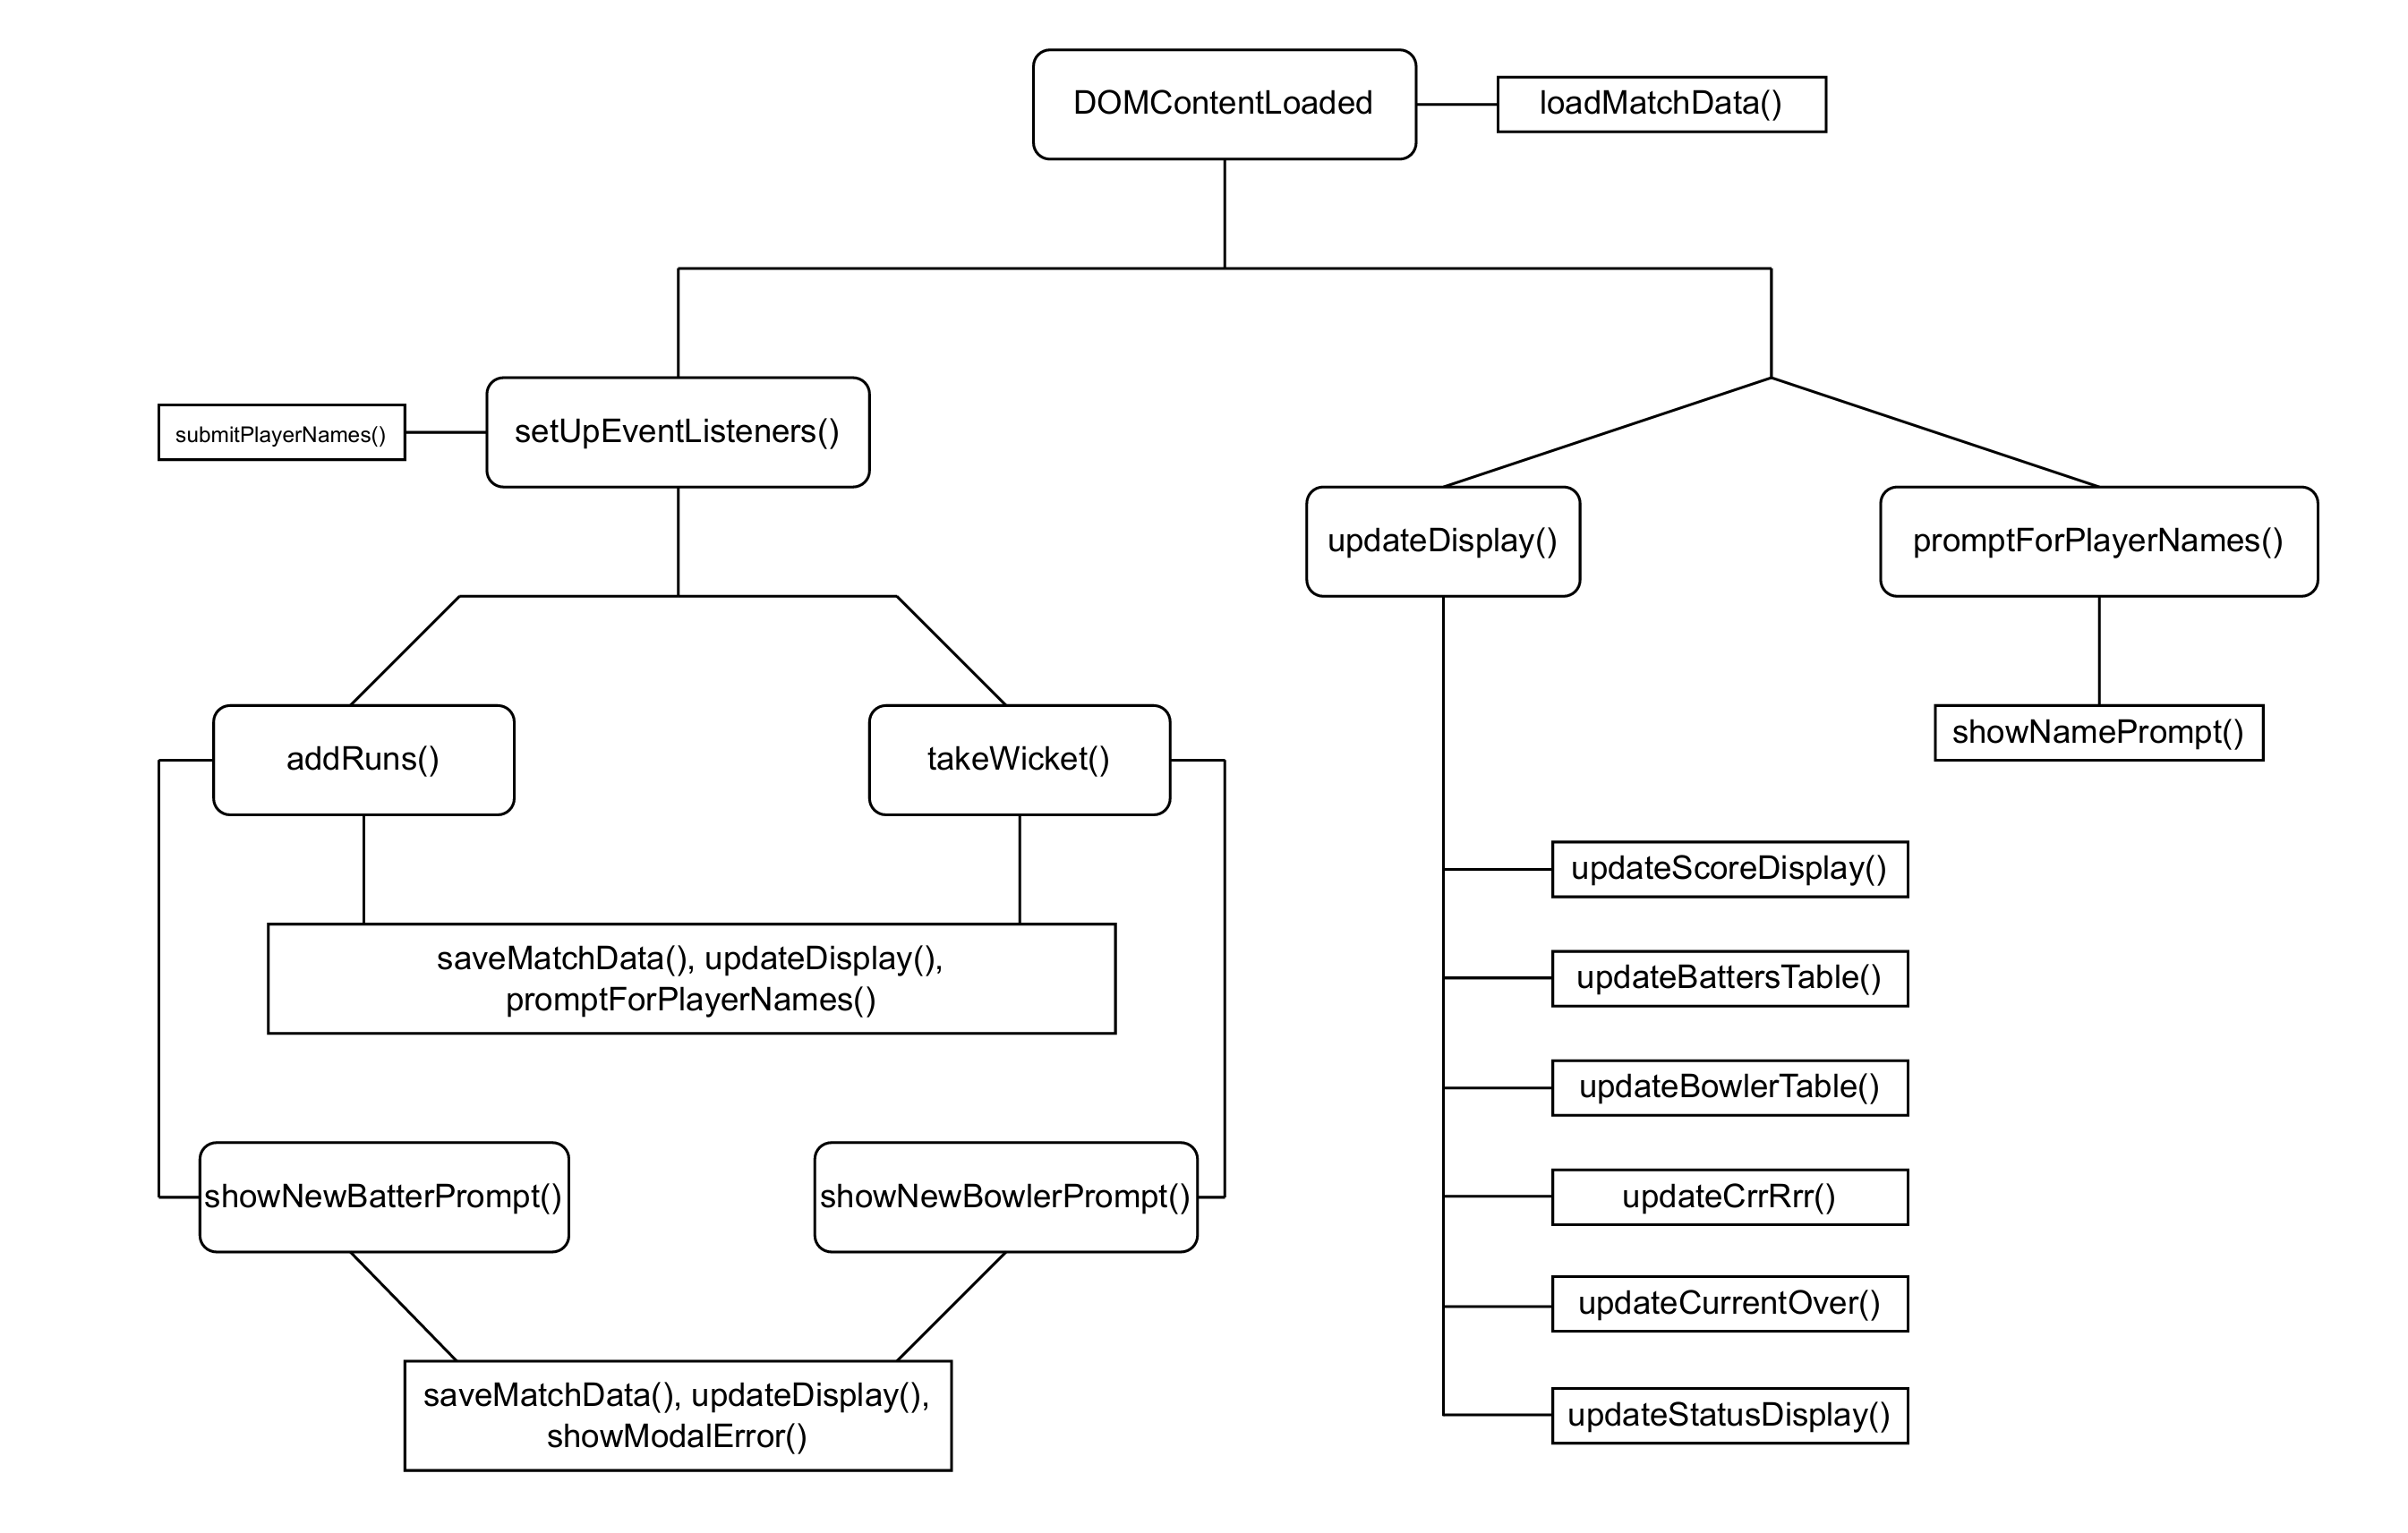
\includegraphics[width=\textwidth]{images/flowchart.png}
\caption{Flowchart Representation of JS Functions in Live Page} 
\label{flowchart}
\end{figure}

\section{References}
\begin{itemize}
  \item \texttt{Background Images:} \url{www.wallpaperflare.com}
  \item \texttt{General AI Chat:} \url{https://chatgpt.com/share/6810c68c-5d30-800b-84c0-c59a2974420f}
  \item \texttt{Design Inspiration:} \url{https://www.espncricinfo.com/} 
\end{itemize}

\end{document}
